\documentclass[]{article}
\usepackage{lmodern}
\usepackage{amssymb,amsmath}
\usepackage{ifxetex,ifluatex}
\usepackage{fixltx2e} % provides \textsubscript
\ifnum 0\ifxetex 1\fi\ifluatex 1\fi=0 % if pdftex
  \usepackage[T1]{fontenc}
  \usepackage[utf8]{inputenc}
\else % if luatex or xelatex
  \ifxetex
    \usepackage{mathspec}
  \else
    \usepackage{fontspec}
  \fi
  \defaultfontfeatures{Ligatures=TeX,Scale=MatchLowercase}
\fi
% use upquote if available, for straight quotes in verbatim environments
\IfFileExists{upquote.sty}{\usepackage{upquote}}{}
% use microtype if available
\IfFileExists{microtype.sty}{%
\usepackage{microtype}
\UseMicrotypeSet[protrusion]{basicmath} % disable protrusion for tt fonts
}{}
\usepackage{hyperref}
\PassOptionsToPackage{usenames,dvipsnames}{color} % color is loaded by hyperref
\hypersetup{unicode=true,
            pdftitle={CS 229 Homework},
            pdfauthor={Tyler Neylon},
            colorlinks=true,
            linkcolor=black,
            citecolor=Blue,
            urlcolor=Blue,
            breaklinks=true}
\urlstyle{same}  % don't use monospace font for urls
\usepackage{graphicx,grffile}
\makeatletter
\def\maxwidth{\ifdim\Gin@nat@width>\linewidth\linewidth\else\Gin@nat@width\fi}
\def\maxheight{\ifdim\Gin@nat@height>\textheight\textheight\else\Gin@nat@height\fi}
\makeatother
% Scale images if necessary, so that they will not overflow the page
% margins by default, and it is still possible to overwrite the defaults
% using explicit options in \includegraphics[width, height, ...]{}
\setkeys{Gin}{width=\maxwidth,height=\maxheight,keepaspectratio}
\IfFileExists{parskip.sty}{%
\usepackage{parskip}
}{% else
\setlength{\parindent}{0pt}
\setlength{\parskip}{6pt plus 2pt minus 1pt}
}
\setlength{\emergencystretch}{3em}  % prevent overfull lines
\providecommand{\tightlist}{%
  \setlength{\itemsep}{0pt}\setlength{\parskip}{0pt}}
\setcounter{secnumdepth}{5}
% Redefines (sub)paragraphs to behave more like sections
\ifx\paragraph\undefined\else
\let\oldparagraph\paragraph
\renewcommand{\paragraph}[1]{\oldparagraph{#1}\mbox{}}
\fi
\ifx\subparagraph\undefined\else
\let\oldsubparagraph\subparagraph
\renewcommand{\subparagraph}[1]{\oldsubparagraph{#1}\mbox{}}
\fi
\usepackage{subfig}
\AtBeginDocument{%
\renewcommand*\figurename{Figure}
\renewcommand*\tablename{Table}
}
\AtBeginDocument{%
\renewcommand*\listfigurename{List of Figures}
\renewcommand*\listtablename{List of Tables}
}
\usepackage{float}
\floatstyle{ruled}
\makeatletter
\@ifundefined{c@chapter}{\newfloat{codelisting}{h}{lop}}{\newfloat{codelisting}{h}{lop}[chapter]}
\makeatother
\floatname{codelisting}{Listing}
\newcommand*\listoflistings{\listof{codelisting}{List of Listings}}

\title{CS 229 Homework}
\author{Tyler Neylon}
\date{345.2016}

% Begin custom, non-pandoc commands.

\newcommand{\latexonlyrule}{\rule}

% End custom, non-pandoc commands.

\begin{document}
\maketitle

\newcommand{\R}{\mathbb{R}}
\newcommand{\eqnset}[1]{\left.\mbox{$#1$}\quad\quad\right\rbrace}
\newcommand{\tr}{\text{tr}\;}
\renewcommand{\th}{\theta}
\newcommand{\toi}{^{(i)}}

These are solutions to the most recent problems posted for Stanford's CS
229 course, as of June 2016. I'm not sure if this course re-uses old
problems, but please don't copy the answers if so. This document is also
available as a
\href{http://tylerneylon.com/notes/cs229/cs229hw.pdf}{pdf}.

\section{Problem set 1}\label{problem-set-1}

\subsection{Logistic regression}\label{logistic-regression}

\subsubsection{Part (a)}\label{part-a}

The problem is to compute the Hessian matrix \(H\) for the function

\[J(\th) = -\frac{1}{m}\sum_{i=1}^m\log(g(y\toi x\toi)),\]

where \(g(z)\) is the logistic function, and to show that \(H\) is
positive semi-definite; specifically, that \(z^THz\ge 0\) for any vector
\(z.\)

We'll use the fact that \(g'(z) = g(z)(1-g(z)).\) We'll also note that
since all relevant operations are linear, it will suffice to ignore the
summation over \(i\) in the definition of \(J.\) I'll use the notation
\(\partial_j\) for \(\frac{\partial}{\partial\th_j},\) and introduce
\(t\) for \(y\th^Tx.\) Then

\[-\partial_j(mJ) = \frac{g(t)(1-g(t))}{g(t)}x_jy = x_jy(1-g(t)).\]

Next

\[-\partial_k\partial_j(mJ) = x_jy\big(-g(t)(1-g(t))\big)x_ky,\]

so that

\[\partial_{jk}(mJ) = x_jx_ky^2\alpha,\]

where \(\alpha = g(t)(1-g(t)) > 0.\)

Thus we can use repeated-index summation notation to arrive at

\[z^THz = z_ih_{ij}z_j = (\alpha y^2)(z_ix_ix_jz_j)
        = (\alpha y^2)(x^Tz)^2 \ge 0.\]

This completes this part of the problem.

\subsubsection{Part (b)}\label{part-b}

Here is a matlab script to solve this part of the problem:

\begin{verbatim}
% problem1_1b.m
%
% Run Newton's method on a given cost function for a logistic
% regression setup.
%

printf('Running problem1_1b.m\n');

% Be able to compute J.
function val = J(Z, theta)
  [m, _] = size(Z);
  g      = 1 ./ (1 + exp(Z * theta));
  val    = -sum(log(g)) / m;
end

% Setup.
X      = load('logistic_x.txt');
[m, n] = size(X);
X      = [ones(m, 1) X];
Y      = load('logistic_y.txt');
Z      = diag(Y) * X;

% Initialize the parameters to learn.
old_theta =  ones(n + 1, 1);
theta     = zeros(n + 1, 1);
i         = 1;  % i = iteration number.

% Perform Newton's method.
while norm(old_theta - theta) > 1e-5
  printf('J = %g\n', J(Z, theta));
  printf('theta:\n');
  disp(theta);
  printf('Running iteration %d\n', i);

  g         = 1 ./ (1 + exp(Z * theta));
  f         = (1 - g);
  alpha     = f .* g;
  A         = diag(alpha);
  H         = Z' * A * Z / m;
  nabla     = Z' * f / m;
  old_theta = theta;
  theta     = theta - inv(H) *  nabla;

  i++;
end

% Show and save output.
printf('Final theta:\n');
disp(theta);
save('theta.mat', 'theta');
\end{verbatim}

Because I have copious free time, I also wrote a Python version. Also
because I'm learning numpy and would prefer to consistently use a
language that I know can produce decent-looking graphs. Here is the
Python script:

\begin{verbatim}
#!/usr/bin/env python

import numpy as np
from numpy import linalg as la


# Define the J function.
def J(Z, theta):
  m, _ = Z.shape
  g    = 1 / (1 + np.exp(Z.dot(theta)))
  return -sum(np.log(g)) / m

# Load data.
X    = np.loadtxt('logistic_x.txt')
m, n = X.shape
X    = np.insert(X, 0, 1, axis=1)  # Prefix an all-1 column.
Y    = np.loadtxt('logistic_y.txt')
Z    = np.diag(Y).dot(X);

# Initialize the learning parameters.
old_theta = np.ones((n + 1,))
theta     = np.zeros((n + 1,))
i         = 1

# Perform Newton's method.
while np.linalg.norm(old_theta - theta) > 1e-5:

  # Print progress.
  print('J = {}'.format(J(Z, theta)))
  print('theta = {}'.format(theta))
  print('Running iteration {}'.format(i))

  # Update theta.
  g         = 1 / (1 + np.exp(Z.dot(theta)))
  f         = 1 - g
  alpha     = (f * g).flatten()
  H         = (Z.T * alpha).dot(Z) / m
  nabla     = Z.T.dot(f) / m
  old_theta = theta
  theta     = theta - la.inv(H).dot(nabla)

  # Update i = the iteration counter.
  i += 1

# Print and save the final value.
print('Final theta = {}'.format(theta))
np.savetxt('theta.txt', theta)
\end{verbatim}

The final value of \(\th\) that I arrived at is

\[\th = (2.62051, -0.76037, -1.17195).\]

The first value \(\th_0\) represents the constant term, so that the
final model is given by

\[y = g(2.62 - 0.76x_1 - 1.17x_2).\]

\subsubsection{Part (c)}\label{part-c}

\begin{figure}[htbp]
\centering
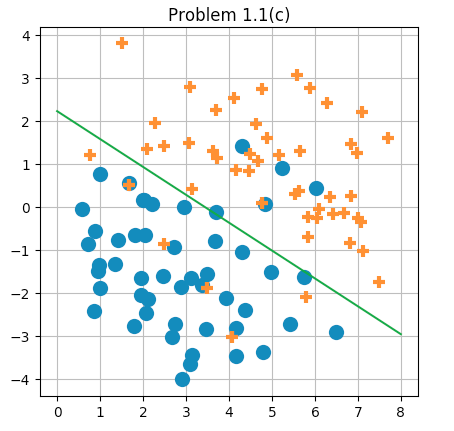
\includegraphics{images/pr1_1c.png}
\caption{The data points given for problem 1.1 along with the decision
boundary learned by logistic regression as executed by Newton's method.}
\end{figure}

\subsection{Poisson regression and the exponential
family}\label{poisson-regression-and-the-exponential-family}

\subsubsection{Part (a)}\label{part-a-1}

Write the Poisson distribution as an exponential family:

\[p(y;\eta) = b(y)\exp\big(\eta^T T(y) - a(\eta)\big),\]

where

\[p(y;\lambda) = \frac{e^{-\lambda}\lambda^y}{y!}.\]

This can be done via

\[\begin{array}{rcl}
\eta & = & \log(\lambda), \\
a(\eta) & = & e^\eta = \lambda, \\
b(y) & = & 1/y!, \text{ and} \\
T(y) & = & y.
\end{array}\]

\subsubsection{Part (b)}\label{part-b-1}

As is usual with generalized linear models, we'll let \(\eta = \th^Tx.\)
The canonical response function is then given by

\[g(\eta) = E[y;\eta] = \lambda = e^\eta = e^{\th^Tx}.\]

\subsubsection{Part (c)}\label{part-c-1}

Based on the last part, I'll define the hypothesis function \(h\) via
\(h(x) = e^{\th^Tx}.\)

For a single data point \((x, y),\) let \(\ell(\th) = \log(p(y|x)) =\)
\(\log(\frac{1}{y!}) + (y\th^T x-e^{\th^Tx}).\) Then

\[\frac{\partial}{\partial\th_j}\ell(\th) = yx_j - x_je^{\th^Tx}
= x_j(y-e^{\th^Tx}).\]

So stochastic gradient ascent for a single point \((x, y)\) would use
the update rule

\[\th := \th + \alpha x(y - h(x)).\]

\subsubsection{Part (d)}\label{part-d}

In section 1.10 of my notes --- the section on generalized linear models
--- I derived the update rule:

\[\th := \th + \alpha\big(T(y)-a'(\th^Tx)\big)x.\]

The missing piece is to proof that \(h(x) = E[y] = a'(\eta),\) which
we'll do next. We'll work in the context of \(T(y)=y,\) as given by the
problem statement. Notice that, for any \(\eta,\)

\[\int p(y)dy = \int b(y)\exp(\eta^Ty - a(\eta))dy = 1.\]

Since this identity is true for all values of \(\eta,\) we can take
\(\frac{\partial}{\partial\eta}\) of it to arrive at the value 0:

\[\begin{array}{rcl}
 0 & = & \frac{\partial}{\partial\eta}\int p(y)dy \\
   & = & \int \frac{\partial}{\partial\eta} b(y)\exp(\eta^Ty - a(\eta))dy \\
   & = & \int b(y)(y - a'(\eta))\exp(\eta^Ty - a(\eta)) dy \\
   & = & \int y p(y)dy - a'(\eta)\int p(y)dy \\
   & = & E[y] - a'(\eta).
\end{array}\]

Thus we can conclude that \(E[y] = a'(\eta) = a'(\th^Tx),\) which
completes the solution.

\subsection{Gaussian discriminant
analysis}\label{gaussian-discriminant-analysis}

\subsubsection{Part (a)}\label{part-a-2}

This problem is to show that a two-class GDA solution effectively
provides a model that takes the form of a logistic function, similar to
logistic regression. This is something I already did in section 2.1 of
\href{http://tylerneylon.com/notes/cs229/cs229.html}{my notes}.

\end{document}
